\documentclass[12pt, a4paper]{article}
\usepackage[utf8]{inputenc}
\usepackage[T1]{fontenc}
\usepackage[english,brazil]{babel}
\usepackage{indentfirst}
\usepackage{graphicx}
\usepackage{amsmath}
\usepackage[left=3cm, top=3cm, right=2cm, bottom=2cm]{geometry}
\usepackage{setspace}
%links%
\usepackage{hyperref}
\setlength{\parindent}{1.25cm}
\graphicspath{ {./} }

\begin{document}
% capa
\begin{titlepage}
\begin{center}
    \large
     {\bf Centro Estadual de Educação Tecnológica Paula Souza} \\
     {\bf Faculdade de Tecnologia Baixada Santista
Rubens Lara} \\ 
    {\bf Curso Superior de Tecnologia em Ciência de Dados} \\
    
    \vspace{215pt}
        {\bf Matemática Básica} \\
    \vspace{10pt}
        {\Large \bf Entropia de Dados}\\
        
    \vspace{100pt}

    \vfill
        {\large  \bf Autores} \\
        {\large  \bf Fernando Gomes Cruz} \\
        {\large \bf Helena Victoria dos Santos Barboza} \\
        {\large \bf Mario Ambrosio De Souza Neto} \\
    \vfill
        \textbf{{\large Santos}\\
        {\large 2023}}
        
\end{center}
\end{titlepage}

\tableofcontents

\newpage

\section{Introdução}

Esse trabalho consiste em demonstrar o cálculo da entropia de dados da "Pesquisa CNT de Opinião - Rodada 158" realizada pela Confederanção Nacional do Transporte em maio de 2023, disponível em 
\begin{center}
\url{ https://cnt.org.br/documento/9ce8872e-b550-4703-87e2-031b075b073b }
\end{center}
que apresenta dados referentes a avaliação do governo no início do 3º mandato do presidente Lula. 

Entropia é um conceito fundamental na teoria da informação e suas aplicações variam em áreas como compressão de dados, criptografia, machine learning, entre outros.

\section{Dados}
Serão utilizado os dados da pesquisa, descritos na página 7 da pesquisa, referentes à 2.002 entrevistas, as quais os entrevistados avaliaram o Governo Federal. Os resultados foram separados em seis classes, com seus valores percentuais:

\begin{itemize}
\item Ótimo - 14,6\%
\item Bom - 28,5\% 
\item Regular - 28,3\%
\item Ruim - 7,8\% 
\item Péssimo - 16,8\% 
\item NS/NR (Não sabem/Não responderam) - 4,0\% 
\end{itemize}

\section{Cálculo da Entropia}
\subsection{Fórmula da Entropia}
A fórmula da entropia é dada por:
$$
H(X) = - \sum_{x \in X} p(x) \log_{} p(x)
$$

\noindent onde,
\begin{itemize}
\item $H(X)$ denota a entropia de uma variável $X$;
\item O somatório é formado por todas as classes $x$ em $X$;
\item $p(x)$ denota a probabilidade de ocorrência de cada classe $x$;
\item A base do logaritmo é usualmente 2, que denota bits de informação.
\item O sinal negativo em frente ao somatório garante que o valor da entropia é não-negativo.
\end{itemize}

\subsection{Cálculo da entropia}
Temos como classes $x$ de $X = \{$Ótimo, Bom, Regular, Ruim, Péssimo, NS/NR$\}$
\\
\begin{itemize}
\item Ótimo - 14,6\% = 0.146
\item Bom - 28,5\% = 0.285
\item Regular - 28,3\% = 0.283
\item Ruim - 7,8\% = 0.078
\item Péssimo - 16,8\% = 0.168
\item NS/NR (Não sabem/Não responderam) - 4,0\% = 0.04
\end{itemize} \\

\newline
\par Cálculo de $\log p(x)$ para cada classe. \\

\newline
$\log_2 0.146 = \frac{\log 0.146}{\log 2} = −2.775959726 \approx -2.78$ \\

$\log_2 0.285 = \frac{\log 0.285}{\log 2} = −1.810966176 \approx -1.81$ \\

$\log_2 0.283 = \frac{\log 0.283}{\log 2} = −1,821126042 \approx -1.82$ \\

$\log_2 0.078 = \frac{\log 0.078}{\log 2} = −3.680382066 \approx -3.68$ \\

$\log_2 0.168 = \frac{\log 0.168}{\log 2} = −2.573466862 \approx -2.57$ \\

$\log_2 0.04 = \frac{\log 0.04}{\log 2} = −4,64385619 \approx -4.64$ \\

Com as classes e os valores de $p(x)$ e $\log p(x)$, podemos verificar o resultado aplicando a fórmula:

$$
\begin{align*}
& H(X) = - (  0.146(−2.78) + 0.285(−1.81) + 0.283(−1,82) \\
& \ ~\ ~\ ~\ + 0.078(-3.68) + 0.168(-2.57) + 0.04(-4.64)) \\
& \ ~\ ~\ ~\  = 2.34119 \\
\end{align*}
$$

Temos como valor de entropia $H(X) = 2.34119$

\subsection{Cálculo da entropia máxima}
Como o conjunto $X$ é composto por seis elementos temos:
$$
maxH(X) = \log_2 6 = 2.58
$$

O valor da entropia máxima é $maxH(X) = 2.58$. \\

Temos que $H(X)$ tem um valor aproximado a $maxH(X)$ indicando que existe um alto nível de aleatoriedade nos dados apresentados.

\subsection{Verificação dos resultados no código Python}
Verifica-se, no código Python, resultados similares aos encontrados no cálculo da entropia dos dados descritos acima. Obtem-se os valores 2.342 de entropia de dados e o valor 2.58 para entropia máxima, como observado na imagem abaixo:
\begin{figure}[h!]
    \caption{Código Python e verificação dos resultados}
    \centering
    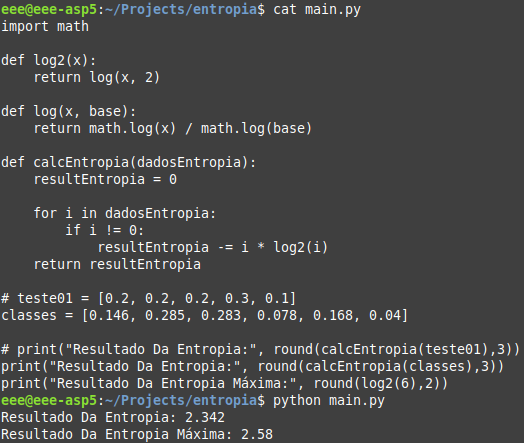
\includegraphics[scale=0.6]{console.png}
\end{figure}
\subsection{Conclusão}
Com base nos resultados obtidos, pode-se concluir que os dados da pesquisa apresentam um grau considerável de diversidade e incerteza nas respostas, indicando uma distribuição variada nas opiniões sobre a avaliação do governo. Isso ressalta a importância de considerar a entropia ao analisar conjuntos de dados e tomar decisões com base nessas informações. Por fim, disponibilizamos o repositório do Github: 
\begin{center}
\url{ https://github.com/feg59crz/entropia}
\end{center}
onde se encontra o arquivo latex 'main.tex' do presente texto e a implementação da fórmula da determinante de qualquer matriz quadrada em um código python 'main.py' e a Figura 1, para que os interessados possam acessar e verificar os resultados obtidos.
\end{document}